\documentclass[tikz]{standalone}

\definecolor{n0}{HTML}{785EF0}
\definecolor{End}{HTML}{DC267F}
\definecolor{Corner}{HTML}{FFB000}
\definecolor{NewHex}{HTML}{648FFF}
\definecolor{Reversal}{HTML}{FE6100}

\begin{document}
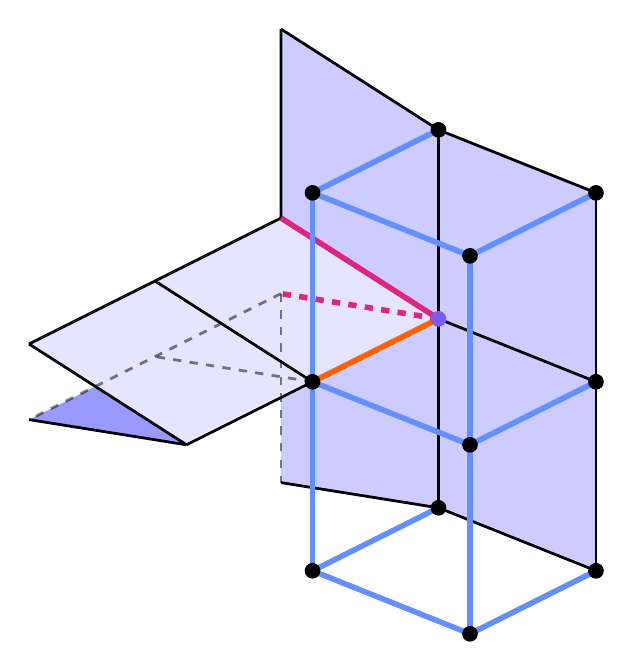
\begin{tikzpicture}[scale=4, x={(0.5cm,-0.2cm)}, y={(0.4cm,0.2cm)}, z={(0.0cm,0.6cm)}]

  %%%%%%%%%% Points pour travailler %%%%%%%%%%

 \coordinate (0) at (0,0,0);
 \coordinate (1) at (1,0,0);
 \coordinate (2) at (1,-1,0);
 \coordinate (3) at (0,-1,0);
 \coordinate (4) at (0,0,1);
 \coordinate (5) at (1,0,1);
 \coordinate (6) at (1,-1,1);
 \coordinate (7) at (0,-1,1);
 \coordinate (8) at (0,0,-1);
 \coordinate (9) at (1,0,-1);
 \coordinate (10) at (1,-1,-1);
 \coordinate (11) at (0,-1,-1);
 \coordinate (12) at (-1,0,-1.2);
 \coordinate (13) at (-1,0,1.2);
 \coordinate (14) at (-1,0,0.2);
 \coordinate (15) at (-1,0,-0.2);
 \coordinate (16) at (-1,-1,-0.2);
 \coordinate (17) at (-1,-2,-0.2);
 \coordinate (18) at (-1,-1,0.2);
 \coordinate (19) at (-1,-2,0.2);
 \coordinate (20) at (0,-2,0);

 
 %%%%%%%%%% Layer blue color %%%%%%%%%%
 \fill [color=blue!40!white] (15) -- (17) -- (20) -- (0) -- cycle ;
 \fill [color=blue!20!white] (0) -- (14) -- (13) -- (4) -- (5) -- (9) -- (8) -- (12) -- (15) -- cycle ;
 \fill [color=blue!10!white] (0) -- (14) -- (19) -- (20) -- cycle ;
 
 %%%%%%%%%%%%%%%% Precedant layer %%%%%%%%%%%%%%%%%%%
 \draw [line width=1] (0) -- (20) ;
 \draw [line width=1] (13) -- (14) -- (19) ;
 \draw [line width=1] (13) -- (4) -- (5) ;
 \draw [line width=1] (0) -- (1) ;
 \draw [line width=1] (12) -- (8) -- (9) ;
 \draw [line width=1] (19) -- (20) ;
 \draw [line width=1] (18) -- (3) ;
 \draw [line width=1] (4) -- (8) ;
 \draw [line width=1] (20) -- (17) ;
 \draw [line width=1] (5) -- (9) ;
 \draw [dashed, line width=1,opacity=0.5] (15) -- (12) ;
 
 \draw [dashed, line width=1,opacity=0.5] (3) -- (16) ;
 \draw [dashed, line width=1,opacity=0.5] (15) -- (17) ;
 
 
 %%%%%%%%%%% Feature edges %%%%%%%%%%%
 \draw [line width=2, color=End] (0) -- (14) ;
 \draw [dashed, line width=2, color=End] (0) -- (15) ;
 \draw [line width=2, color=Reversal] (0) -- (3) ;

 %%%%%%%%%%% Faces %%%%%%%%%%%
 \draw [opacity=0] (0) -- (13) ;
 \draw [opacity=0] (0) -- (12) ;
 \draw [opacity=0] (0) -- (5) ;
 \draw [opacity=0] (0) -- (9) ;
 \draw [opacity=0] (0) -- (18) ;
 \draw [opacity=0] (0) -- (16) ;
 
 %%%%%%%%%%% The HEXAS created %%%%%%%%%%% 
 \draw [line width=2, color=NewHex] (4) -- (7) -- (6) -- (5) ;
 \draw [line width=2, color=NewHex] (1) -- (2) -- (3) ;
 \draw [line width=2, color=NewHex] (8) -- (11) -- (10) -- (9) ;
 \draw [line width=2, color=NewHex] (7) -- (11) ;
 \draw [line width=2, color=NewHex] (6) -- (10) ;

  %%%%%%%%%%% HEXA NODES %%%%%%%%%%%
 \draw (0) node[circle, fill=n0, inner sep = 2 pt] {};
 
  \foreach \i in {1,...,11}
 {
   \draw (\i) node[circle, fill=black, inner sep = 2 pt] {};
 }

\end{tikzpicture}
\end{document}